\PassOptionsToPackage{table}{xcolor}

% \documentclass[usenames,dvipsnames]{beamer}
\documentclass[usenames,dvipsnames,aspectratio=169]{beamer}
% \usepackage{helvet}
\usepackage{appendixnumberbeamer}
%Helveltica
\usepackage{adjustbox,graphicx,url,hyperref,multirow,makecell,caption,subcaption}
\usepackage{mathtools}
\usepackage{listings}
\usepackage[normalem]{ulem}
\usepackage[percent]{overpic}
\usepackage{fancybox}
\usepackage{amssymb}
\usepackage{amsmath}

\usepackage{fontspec}
\setmainfont{Rubik-Light.ttf}[
BoldFont = Rubik-Medium.ttf ,
ItalicFont = Rubik-LightItalic.ttf ,
BoldItalicFont = Rubik-MediumItalic.ttf]

\definecolor{crimsonred}{RGB}{153,29,29}
\definecolor{darkgray_instructors}{RGB}{150,150,150}

\usepackage{tikz}
\usetikzlibrary{mindmap}
\usetikzlibrary{
  angles,
  arrows,
  arrows.meta,
  calc,
  intersections,
  positioning,
  quotes,
  shapes.geometric,
  through,
}

\newlength{\newTextWidth}
\newlength{\newMinWidth}
\newlength{\newMinHeight}
\setlength{\newTextWidth}{2.9cm}
\setlength{\newMinWidth}{0.16\textwidth}
\setlength{\newMinHeight}{0.14\textheight}

\newcommand\HighlightedNode{none}
\newcommand\Highlight[1]{\renewcommand\HighlightedNode{#1}}

\makeatletter 

\long\def\ifnodedefined#1#2#3{%
    \@ifundefined{pgf@sh@ns@#1}{#3}{#2}%
}
\makeatother

\newcommand\methodologyFig{
    \begin{tikzpicture}[
        body/.style={
            rectangle, % shape
            very thick, % border
            draw=white!30!UniTangerina!70, % outline
            % top color=white,
            top color=white!70!UniTangerina!30,
            bottom color=white!70!UniTangerina!30,
            font=\small, % Font
            align=center,
            x=0em,
            y=0em,
            node distance=.8em,
            >=stealth'
        }]
        
        \node (P1) [body, text width=\newTextWidth, minimum height=\newMinHeight, minimum width=\newMinWidth] 
        {\hyperlink{P1}{Part 1}};
        
        \node (P2) [body, below=of P1, text width=\newTextWidth, minimum height=\newMinHeight, minimum width=\newMinWidth]
        {\hyperlink{P2}{Part 2}};
        
        \node (P3) [body, below=of P2, text width=\newTextWidth, minimum height=\newMinHeight, minimum width=\newMinWidth]
        {\hyperlink{P3}{Part 3\\(\textbf{Click Here})}};
        
        \node (P4) [body, below=of P3, text width=\newTextWidth, minimum height=\newMinHeight, minimum width=\newMinWidth]
        {\hyperlink{P4}{Part 4}};
        
        \node (P5) [body, below=of P4, text width=\newTextWidth, minimum height=\newMinHeight, minimum width=\newMinWidth]
        {\hyperlink{P5}{Part 5}};
        
        \path (P1) edge[->] (P2);
        \path (P2) edge[->] (P3);
        \path (P3) edge[->] (P4);
        \path (P4) edge[->] (P5);
        
        \ifnodedefined{\HighlightedNode}{
            \draw [ultra thick,UniTangerina,dashed] (\HighlightedNode.center) circle [x radius=4.7em,y radius=1.8em];
            }{}
        
    \end{tikzpicture}}


\lstset{
  basicstyle=\footnotesize\ttfamily,
  keywordstyle=\bfseries,
  breaklines=false,
  keepspaces=true,
  frame=lrtb,
  abovecaptionskip=0pt,
  aboveskip=\smallskipamount,
  belowcaptionskip=0pt,
  belowskip=\smallskipamount,
  captionpos=b,
  numbers=left,
  numberstyle=\tiny,
  numbersep=5pt,
  upquote
}

\usepackage[utf8]{inputenc}
% \usepackage{subfigure}
\usepackage{verbatim}
\usepackage[brazil]{babel}
\usetheme{uniud}
\newtheorem{thm}{Teorema}
\DeclareMathOperator{\argmin}{argmin}
\DeclareMathOperator{\argmax}{argmax}


%%% Bibliography
\usepackage[backend=biber]{biblatex}
\usepackage{float}


\addbibresource{bibliography.bib}

% Author names in publication list are consistent 
% i.e. name1 surname1, name2 surname2
% See https://tex.stackexchange.com/questions/106914/biblatex-does-not-reverse-the-first-and-last-names-of-the-second-author
\DeclareNameAlias{author}{first-last}

%%% Suppress biblatex annoying warning
\usepackage{silence}
\WarningFilter{biblatex}{Patching footnotes failed}

%%% Some useful commands
% pdf-friendly newline in links
\newcommand{\pdfnewline}{\texorpdfstring{\newline}{ }} 
% Fill the vertical space in a slide (to put text at the bottom)
\newcommand{\framefill}{\vskip0pt plus 1filll}
\newcommand{\oifo}{\textsc{OInvOnline-FO}}
\newcommand{\oild}{\textsc{OInvOnline-LD}}

\title[email@inf.puc-rio.br]{TITLE}

\author[Student Name]{
 \textbf{Student Name}
  \pdfnewline
  Simone D. J. Barbosa (advisor)
  \pdfnewline
}

\newcommand\email{email@inf.puc-rio.br}

\institute{Pontifícia Universidade Católica do Rio de Janeiro}
% \date{Rio de Janeiro, 05 de setembro de 2020}
\date{September 5, 2020}

\begin{document}

\begin{frame}
\titlepage
\end{frame}

% % \begin{frame}{Agenda}
% \begin{frame}{Content}
% \tableofcontents
% \end{frame}


\section{Section 1}
\framecard[UniTangerina]{Section 1}
%------------------------------------------------
\begin{frame}{Section 1}

\begin{figure}[H]
\centering
  \centering
  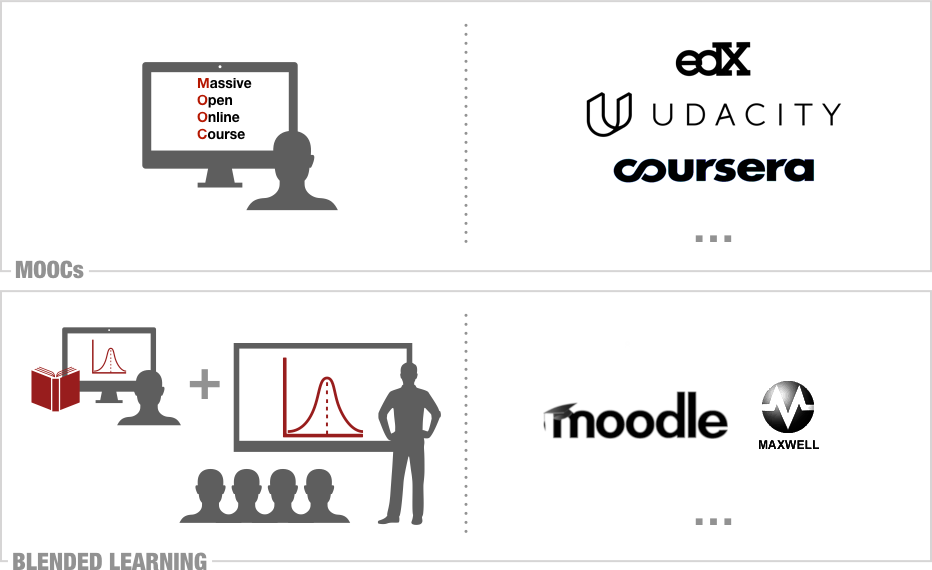
\includegraphics[width=.75\linewidth]{figures/Distance_Learning.png}
\end{figure}

\end{frame}

%------------------------------------------------
\begin{frame}{Section 1}

\centering
\begin{overpic}[width=.75\linewidth]{figures/Flexibility.png}
 \put (78,28) 
 	{%\colorbox{white}
      {\parbox{.7\linewidth}{%
      \textcolor{crimsonred}{\textbf{\textbf{BOLD TEXT}}}
      }
      }
	}
 \put (6,-3) 
 	{%\colorbox{white}
      {\parbox{.7\linewidth}{%
      \textcolor{crimsonred}{\textbf{\textit{Another text}}}
      }
      }
	}
 \put (38,-3) 
 	{%\colorbox{white}
      {\parbox{.7\linewidth}{%
      \textcolor{crimsonred}{TEXT}
      }
      }
	}
%   \caption{Caption.}
\end{overpic}

\end{frame}

%------------------------------------------------
\begin{frame}
\frametitle{Section 1}

“\textit{Some Citation}”
\begin{itemize}
    \item \footnotesize{Reference}
\end{itemize}

\vspace*{0.9cm}

A text
\begin{itemize}
    \item Item
    \begin{itemize}
        \item Sub Item
        \item Another Item
        \begin{itemize}
            \item Details
        \end{itemize}
    \end{itemize}
\end{itemize}


\end{frame}
%------------------------------------------------
\begin{frame}
\frametitle{Research Question}

\centering
\begin{overpic}[width=.75\linewidth]{figures/Logs_analyses_tool.png}
 \put (-16,40) 
 	{%\colorbox{white}
      {\parbox{\linewidth}{%
        \begin{block}{Research Question}
        \end{block}
      }
      }
	}
\end{overpic}

\end{frame}
%------------------------------------------------
\section{Section 2}
\framecard[UniTangerina]{Section 2 (Tangerina Background)}
%------------------------------------------------
\begin{frame}{Methodology}

\vspace*{-0.38cm}
\hspace*{-0.625cm}
\methodologyFig

\end{frame}
%------------------------------------------------
\begin{frame}{Part 1}
\label{P1}

\vspace*{-1.00cm}
\begin{columns}[t]
    \column{.129\textwidth}
        \Highlight{P1}
        \methodologyFig
    
    \column{.1\textwidth}
    
    \column{.82\textwidth}
        \begin{block}{Part 1}
        \small{
            Some Consideration.
        }
        \end{block}
    
    
\end{columns}

\end{frame}
%------------------------------------------------
\begin{frame}{Part 1}
\label{part1}

\vspace*{-1.00cm}
\begin{columns}[t]
    \column{.129\textwidth}
        \Highlight{P1}
        \methodologyFig
    
    \column{.1\textwidth}
    
    \column{.82\textwidth}
        \begin{itemize}
            \item Item 1
        \end{itemize}
        
        \begin{itemize}
            \item \hyperlink{methodology1:mapping}{(\textbf{Click Here})}
        \end{itemize}
        
\end{columns}

\end{frame}

%------------------------------------------------
\begin{frame}{Part 2}
\label{P2}

\vspace*{-0.86cm}
\begin{columns}[t]
    \column{.129\textwidth}
        \Highlight{P2}
        \methodologyFig
    
    \column{.1\textwidth}
    
    \column{.82\textwidth}
        \begin{block}{Part 2}
        \small{
            Some Consideration
        }
        \end{block}
\end{columns}

\end{frame}
%------------------------------------------------
\begin{frame}{Part 3}
\label{P3}

\vspace*{-0.86cm}
\begin{columns}[t]
    \column{.129\textwidth}
        \Highlight{P3}
        \methodologyFig
    
    \column{.1\textwidth}
    
    \column{.82\textwidth}
        \begin{block}{Part 3}
    \small{
        Some Consideration
    }
    \end{block}
\end{columns}

\end{frame}

%------------------------------------------------
\begin{frame}{Part 4}
\label{P4}

\vspace*{-0.857cm}
\begin{columns}[t]
    \column{.129\textwidth}
        \Highlight{P4}
        \methodologyFig
    
    \column{.1\textwidth}
    
    \column{.82\textwidth}
        \begin{block}{Part 4}
    
    \end{block}
\end{columns}

\end{frame}
%------------------------------------------------
\begin{frame}{Part 5}
\label{P5}

\vspace*{-0.765cm}
\begin{columns}[t]
    \column{.129\textwidth}
        \Highlight{P5}
        \methodologyFig
    
    \column{.1\textwidth}
    
    \column{.82\textwidth}

        \small{
            \begin{itemize}
                \item A table
            \end{itemize}
            
            \definecolor{darkgray}{RGB}{204,204,204}
\definecolor{gray}{RGB}{217,217,217}
\definecolor{lightgray}{RGB}{239,239,239}
\definecolor{white}{RGB}{255,255,255}

\arrayrulecolor{white}

\setlength\tabcolsep{2.2pt} % space between the text and the left/right border. Default Value = 6.0pt

\begin{table} [!h]
  \centering
  \label{tab:models_prediction}
  
  \begin{tabular}{l|r|r|r}

  \rowcolor{lightgray}  
    \cellcolor{gray}Method & \textbf{Decision Tree} & Logistic Regression & Random Forest\\

    \hline
    \hline
    
    \cellcolor{gray}Prec.(\%) & \textbf{81.93} & 69.62 & 78.93 \\

    \hline
    \hline
        
  \rowcolor{lightgray}
    \cellcolor{gray}Rec.(\%) & \textbf{78.33} & 70.39 & 75.53 \\
    
    \hline
    \hline
    
    \cellcolor{gray}F1(\%) & \textbf{78.08} & 66.36 & 75.20 \\

  \hline
  \end{tabular}
\end{table}


        }
       
    \end{columns}

\end{frame}

%------------------------------------------------
\begin{frame}{Title}

    \vspace*{-1.28cm}
\begin{columns}[t]
    \column{.45\textwidth}
        \begin{itemize}
            \item Item 1
            \begin{itemize}
                \item Sub Item 1
            \end{itemize}
            \begin{itemize}
                \item Sub Item 2
            \end{itemize}
            \begin{itemize}
                \item Sub Item 3
            \end{itemize}
        \end{itemize}
        
        \begin{itemize}
            \item Item 2
        \end{itemize}

    \column{.5\textwidth}
        \vspace*{0.28cm}
        \centering
        \begin{overpic}[width=\linewidth]{figures/instructor.jpeg}
        \end{overpic}
   
\end{columns}

\end{frame}

\section{Section 3}
\framecard[UniGrafite]{Section 3 (Grafite Background)}
%------------------------------------------------
\begin{frame}{Section 3}

\vspace*{-.29cm}
    
    \centering
    \begin{overpic}[width=.535\linewidth]{figures/likert_evaluate_topics_en.png}
        \put(0,0)
            {\color{red} \linethickness{0mm}
                \frame{
\includegraphics[width=.535\linewidth]{figures/likert_evaluate_topics_en_highlight.png}}
            }
        
        \scriptsize
        \put (-145.5,42.5) 
         	{%\colorbox{white}
              {\parbox{.8\linewidth}{%
                \raggedleft \textbf{Highlight:} Look these results,\\audience.
              }
              }
        	}
    \end{overpic}
    
\end{frame}

\section{Section 4}
\framecard[UniMarfim]{Section 4 (Marfim Background)}
%------------------------------------------------
\begin{frame}{Section 4}

\begin{itemize}
\item Statement 1
\end{itemize}

\begin{itemize}
\item Statement 2
\end{itemize}

\end{frame}


% ######################################################################
\appendix
%------------------------------------------------
\framecard[UniTangerina]{Appendix}

\begin{frame}
\frametitle{Further Information}
\label{methodology1:mapping}

\begin{itemize}
    \item \href{https://www.google.com/}{\textbf{Click Here} to open Google}
\end{itemize}

\begin{figure}[h!]
% \centering
\hspace*{5cm}

\begin{overpic}[width=.5\linewidth]{figures/fig_problems.png}
%%%%%%%%%%%%%%%%%%%%%%%%%  
    \small
    \put (76.5,93.3) 
     	{%\colorbox{white}
          {\parbox{.7\linewidth}{%
          \textcolor{white}{ \textbf{64}}
          }
          }
    	}
    \scriptsize
    \put (-134.5,93.5) 
     	{%\colorbox{white}
          {\parbox{.8\linewidth}{%
            \raggedleft \textbf{Item 1}
          }
          }
    	}
%%%%%%%%%%%%%%%%%%%%%%%%%  
    \small
    \put (43,80.7) 
     	{%\colorbox{white}
          {\parbox{.7\linewidth}{%
          \textcolor{white}{\textbf{38}}
          }
          }
    	}
    \scriptsize
    \put (-134.5,80.7) 
     	{%\colorbox{white}
          {\parbox{.8\linewidth}{%
            \raggedleft \textbf{Item 2}
          }
          }
    	}
%%%%%%%%%%%%%%%%%%%%%%%%%  
    \small
    \put (25,67.8) 
     	{%\colorbox{white}
          {\parbox{.7\linewidth}{%
          \textcolor{white}{\textbf{24}}
          }
          }
    	}
    \scriptsize
    \put (-134.5,67.8) 
     	{%\colorbox{white}
          {\parbox{.8\linewidth}{%
            \raggedleft Item 3
          }
          }
    	}
%%%%%%%%%%%%%%%%%%%%%%%%%  
    \small
    \put (22,55.2)
     	{%\colorbox{white}
          {\parbox{.7\linewidth}{%
          \textcolor{white}{\textbf{22}}
          }
          }
    	}
    \scriptsize
    \put (-134.5,55.2)
     	{%\colorbox{white}
          {\parbox{.8\linewidth}{%
            \raggedleft Item 4
          }
          }
    	}
%%%%%%%%%%%%%%%%%%%%%%%%%  
    \small
    \put (12,42.3)
     	{%\colorbox{white}
          {\parbox{.7\linewidth}{%
            \textcolor{white}{\textbf{14}}
          }
          }
    	}
    \scriptsize
    \put (-134.5,42.3)
     	{%\colorbox{white}
          {\parbox{.8\linewidth}{%
            \raggedleft Item 5
          }
          }
    	}
%%%%%%%%%%%%%%%%%%%%%%%%%  
    	\put (27,35.5)
     	{%\colorbox{white}
          {\parbox{.7\linewidth}{%
            Number of \colorbox{crimsonred}{\textcolor{white}{\textbf{Results}}}
          }
          }
    	}
%   \caption{Overall results.}
\end{overpic}
\end{figure}

\vspace*{-95pt}
\hyperlink{part1}{\beamerreturnbutton{} back}

\end{frame}

%------------------------------------------------
\begin{frame}[plain]
  \centering
  \noindent\makebox[\textwidth]{
    \begin{overpic}[width=\paperwidth]{figures/darth.jpg}
     \put (15,40)
     	{
          {\parbox{\linewidth}{%
            \Huge{\textcolor{white}{\textbf{Enjoy!}}}
          }
          }
    	}
    \end{overpic}
    }

\end{frame}

\end{document}